\documentclass[printmode, oneside]{pwr}
%opcje klasy dokumentu mgr.cls zostały opisane w dołączonej instrukcji

%poniżej deklaracje użycia pakietów, usun±ć to co jest niepotrzebne
\usepackage{polski}       %przydatne podczas składania dokumentów w
%j. polskim 
%\usepackage[polish]{babel} %alternatywnie do pakietu
%polski, wybrać jeden z nich
\usepackage[utf8]{inputenc} %kodowanie znaków, zależne od systemu
\usepackage[T1]{fontenc} %poprawne składanie polskich czcionek

%pakiety do grafiki
\usepackage{graphicx}
\usepackage{subfigure}
\usepackage{psfrag}

%pakiety dodające dużo dodatkowych poleceń matematycznych
\usepackage{amsmath}
\usepackage{amsfonts}

%pakiety wspomagające i poprawiające składanie tabel
\usepackage{supertabular}
\usepackage{array}
\usepackage{tabularx}
\usepackage{hhline}

%pakiet wypisuj±cy na marginesie etykiety równań i rysunków
%zdefiniowanych przez \label{}, chc±c wygenerować finaln± wersję
%dokumentu wystarczy usunąć poniższ± linię
\usepackage{showlabels}

%definicje własnych poleceń
\newcommand{\R}{I\!\!R} %symbol liczb rzeczywistych, działa tylko w
                        %trybie matematycznym
\newtheorem{theorem}{Twierdzenie}[section] %nowe otoczenie do
                                           %składania twierdzeń

%dane do złożenia strony tytułowej
\title{Six Sigma (TODO)}
\engtitle{\ }
\author{
\bigskip
\begin{minipage}{2in}
\vfil
\mbox{Radosław Grymin (180499)}\\
\mbox{Karol Wons (172222)}
\end{minipage}
}

\supervisor{dr inż. Andrzej Rusiecki}
%\guardian{dr hab. inż. Imię Nazwisko Prof. PWr, I-6} %nie używać
%je¶li opiekun jest t± sam± osob± co prowadz±cy pracę

\date{2013} %standardowo u dołu strony tytułowej umieszczany jest
%bież±cy rok, to polecenie pozwala wstawić dowolny rok

%poniżej jest lista kierunków i specjalności na wydziale elektroniki,
%należy wybrać wła¶ciwe lub dopisać jeśli nie ma odpowiednich
\field{Automatyka i Robotyka (AIR)}
\specialisation{Technologie Informacyjne\\ w Systemach Automatyki (ART)}

\begin{document}
\bibliographystyle{plabbrv} %tylko gdy używamy BibTeXa, ustawia polski
                            %styl bibliografii

\maketitle %polecenie generuj±ce stronę tytułową 

\tableofcontents %spis treści
 % wstawia pierwsze strony takie jak strona tytulowa,
                   % spis tresci, dedykacja
                   

% Tu zaczyna sie                  
\chapter{Opis projektu}
\section{Cel projektu}
  Celem projektu jest poznanie i zastosowanie statystycznych metod
wspomagających podejmowanie decyzji w metodyce zarządzania Lean Six Sigma.
Do badań użyto środowiska Minitab (skorzystano z licencji pracowniczej 
Radosława Grymina).

\section{Zarys projektu}
  Projekt będzie składał się z dwóch części: teoretycznego
opisu metodyki Six Sigma oraz
przeprowadzeniu doświadczeń na przykładowych danych.

Wdrażanie metodologii Six Sigma do działającego procesu
skupia się na iteracyjnym cyklu DMAIC (ang. \textit{Define, Measure, Analyze, Improve and Control}) bazującym na pomiarach działania procesu, statystycznej analizy i stałych 
popraw.

Doświadczenia przeprowadzane będą w programie Minitab wspierającym analizę statystyczną procesu.

\chapter{Harmonogram pracy}
	Prace nad projektem rozpoczynają się z dniem 23.10.2013 (początek tygodnia I).

\begin{itemize}
	\item \textbf{Tydzień I-II:} Zapoznanie się z tematyką Six Sigma, poszukiwanie literatury,
	zapoznanie się za środowiskiem Minitab,
	\item \textbf{Tydzień III-V:} Sporządzenie teoretycznego opisu metodyki Six Sigma.
	Konsultacje z prowadzącym.
	\item \textbf{Tydzień V-VII:} Wygenerowanie danych i dokonanie ich analizy.
	\item \textbf{Tydzień VIII:} Przedstawienie wyników prowadzącemu.
	\item \textbf{Tydzień VIII-X:} Ewentualne poprawki projektu.
\end{itemize}
	
\chapter{Wprowadzenie do Lean Six Sigma}
	Lean Six Sigma jest sprawdzoną metodologią usprawniania procesów
sterowaną przez potrzeby biznesowe oraz wymagania klientów.
Opiera się na danych pobieranych z procesu.

Lean Six Sigma skupia w sobie metodykę lean, która skupia się na redukcji wszelkiego
marnotrawstwa z procesu i usprawnianiu produktywności oraz Six Sigma, która skupia się 
na redukcji wariancji oraz defektów.

Termin Sigma odnosi się do statystycznej miary określającej jak daleko wyjście procesu zbacza
od jego celu  lub wymagań klienta.

\section{Skrócona historia Lean Six Sigma}
	We wczesnych latach 50' XX wieku, firma Toyota stworzyła System produkcyjny Toyoty (ang. \emph{Toyota Production System})
bazujący na wcześniejszych doświadczeniach związanych z usuwaniem marnotrawstwa i ciągłym
udoskonalaniem procesu. System produkcyjny Toyoty jest uważany za prekursora metodyki Lean. Kładł on nacisk na pozbywanie się marnotrawstwa (ang. \textit{removal of waste}), usprawnianie przepływu (ang. \textit{improving flow}) oraz 
poprawianie ogólnej oceny produktu z puntu widzenia klienta (ang. \emph{customer value}).

Six Sigma zrodziła się w firmie Motorola w latach 80' XX wieku. Stworzył ją 
dyrektor generalny Motoroli w trakcie realizacji wyzwania polegającego na dziesięciokrotnym udoskonaleniu jakości produktów w ciągu pięciu lat.
W trakcie, gdy kierownicy Motoroli szukali sposobu, żeby uzyskać ten cel, inżynier
Bill Smith analizował korelację pomiędzy czasem życia produktu, a tym jak często 
produkt był naprawiany w trakcie produkcji.
\begin{figure}[!htp]
	\centering
	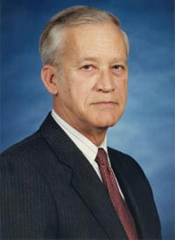
\includegraphics[width=0.25\textwidth]{img/bill-smith2}
	\caption{Bill Smith znany jako ,,Ojciec metodologii Six Sigma''}
\end{figure}
Wykazał, że jeżeli produkt
został uznany za uszkodzony i został naprawiony w czasie produkcji, inne
usterki zostawały przeoczone i ujawniały się we wczesnym okresie użytkowania przez klienta. Jeżeli natomiast produkt został uznany za sprawny, rzadko pojawiały się 
w nim wady u klienta. Doprowadziło to do narodzin metodologii Six Sigma.
Początkowo Six Sigma było zwyczajną metryką, miarą jakości procesu.
Six Sigma to pogoń za jakością określającą nie więcej niż 3,4 usterek na milion sposobności
(ang. 3.4\emph{DPMO}, \emph{Defects Per Milion Opportunities}).

Do roku 1993 Motorola osiągnęła poziom jakości Six Sigma w każdym zakładzie produkcyjnym.
Pozostałe firmy zaczęły brać udział w rewolucji jakościowej ---
Honeywell (później Allied Signal), Texas Instruments, Eastman Kodak jako pierwsze
zaadoptowały metodykę Six Sigma u siebie we wczesnych latach 90' XX wieku.
Stworzono metodę MAIC (ang. \textit{Measure, Analyze, Improve and Control}) służącą
do  wdrażania metodologii Six Sigma do istniejącego procesu.

W 1995 roku, General Electrics zaczął korzystać z Six Sigma. Dyrektor generalny
GE Jack Welch stał się jednym z największych obrońców tej metodyki.
\begin{figure}[!htp]
	\centering
	
\includegraphics[width=0.25\textwidth]{img/welch}
	\caption{Dyrektor generalny General Electrics --- Jack Welch}
\end{figure}
GE wprowadziło również fazę \emph{Define} jako pierwszą fazę do metody MAIC (tak powstao \textit{DMAIC}). Do roku 
2001, firma GE odnotowała oszczędność 4,5 biliona dolarów jako bezpośredni
rezultat działania Six Sigma.

Ostatecznie, na początku pierwszej dekady XXI w., wiele firm zaczęło łączyć metodyki Lean oraz Six Sigma we wszechstronną metodologię usprawnieniową znana obecnie jako Lean Six Sigma.

\section{Czym jest Lean?}
	Lean jest systematyczną metodologią eliminacji marnotrawstwa lub eliminacji pracy niemającej wpływu
na wartość produktu (z perspektywy klienta, ang \emph{non-value added work}) 
oraz maksymalizacji wartości.
Lean zewnętrznie skupia się na maksymalizacji wartości z perspektywy klienta, a wewnętrznie na eliminacji marnotrawstwa oraz powiązanych kosztów procesu.

Lean jest 



% \appendix
% \chapter{Donec cursus nulla vitae pede}


% \addcontentsline{toc}{chapter}{Bibliografia} %utworzenie w
                                             %spisie treści pozycji
                                             %Bibliografia

% \bibliography{bibliografia} % wstawia bibliografię korzystaj±c z pliku
                            % bibliografia.bib - dotyczy BibTeXa,
                            % jeżeli nie korzystamy z BibTeXa należy
                            % użyć otoczenia thebibliography

%opcjonalnie może się tu pojawić spis rysunków i tabel
% \listoffigures
% \listoftables
\end{document}

